 \documentclass[12pt, oneside]{article}

\usepackage[letterpaper, scale=0.89, centering]{geometry}
\usepackage{fancyhdr}
\setlength{\parindent}{0em}
\setlength{\parskip}{1em}

\pagestyle{fancy}
\fancyhf{}
\renewcommand{\headrulewidth}{0pt}
\rfoot{\href{https://creativecommons.org/licenses/by-nc-sa/2.0/}{CC BY-NC-SA 2.0} Version \today~(\thepage)}

\usepackage{amssymb,amsmath,pifont,amsfonts,comment,enumerate,enumitem}
\usepackage{currfile,xstring,hyperref,tabularx,graphicx,wasysym}
\usepackage[labelformat=empty]{caption}
\usepackage[dvipsnames,table]{xcolor}
\usepackage{multicol,multirow,array,listings,tabularx,lastpage,textcomp,booktabs}

\lstnewenvironment{algorithm}[1][] {   
    \lstset{ mathescape=true,
        frame=tB,
        numbers=left, 
        numberstyle=\tiny,
        basicstyle=\rmfamily\scriptsize, 
        keywordstyle=\color{black}\bfseries,
        keywords={,procedure, div, for, to, input, output, return, datatype, function, in, if, else, foreach, while, begin, end, }
        numbers=left,
        xleftmargin=.04\textwidth,
        #1
    }
}
{}
\lstnewenvironment{java}[1][]
{   
    \lstset{
        language=java,
        mathescape=true,
        frame=tB,
        numbers=left, 
        numberstyle=\tiny,
        basicstyle=\ttfamily\scriptsize, 
        keywordstyle=\color{black}\bfseries,
        keywords={, int, double, for, return, if, else, while, }
        numbers=left,
        xleftmargin=.04\textwidth,
        #1
    }
}
{}

\newcommand\abs[1]{\lvert~#1~\rvert}
\newcommand{\st}{\mid}

\newcommand{\A}[0]{\texttt{A}}
\newcommand{\C}[0]{\texttt{C}}
\newcommand{\G}[0]{\texttt{G}}
\newcommand{\U}[0]{\texttt{U}}

\newcommand{\cmark}{\ding{51}}
\newcommand{\xmark}{\ding{55}}

 
\begin{document}
        
        
        \begin{multicols}{2}
\begin{center}\begin{tabular}{cc|c}
Inputs &  & Output \\
$x$ & $y$ & $x \text{ AND } y$  \\
\hline
$1$ & $1$ & $1$\\
$1$ & $0$ & $0$\\
$0$ & $1$ & $0$\\
$0$ & $0$ & $0$\\
\end{tabular}\end{center}
\columnbreak
\begin{center}\includegraphics[height=0.6in]{../../resources/images/xANDy.png} \end{center}
\end{multicols}
\begin{multicols}{2}
\begin{center}\begin{tabular}{cc|c}
Inputs &  & Output \\
$x$ & $y$ & $x \text{ XOR } y$  \\
\hline
$1$ & $1$ & $0$\\
$1$ & $0$ & $1$\\
$0$ & $1$ & $1$\\
$0$ & $0$ & $0$\\
\end{tabular}\end{center}
\columnbreak
\begin{center}\includegraphics[height=0.4in]{../../resources/images/xXORy.png} \end{center}
\end{multicols}
\begin{multicols}{2}
\begin{center}\begin{tabular}{c|c}
Input  & Output \\
$x$ & $\text{NOT } x$  \\
\hline
$1$ & $0$\\
$0$ & $1$\\
\end{tabular}\end{center}
\columnbreak
\begin{center}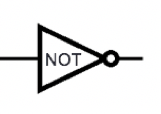
\includegraphics[height=0.5in]{../../resources/images/NOTx.png} \end{center}
\end{multicols}
% \begin{center}
%     \begin{tabular}{p{2in}p{2in}p{2in}}
%     \begin{center}\begin{tabular}{cc|c}
%     Inputs &  & Output \\
%     $x$ & $y$ & $x \text{ AND } y$  \\
%     \hline
%     $1$ & $1$ & $1$\\
%     $1$ & $0$ & $0$\\
%     $0$ & $1$ & $0$\\
%     $0$ & $0$ & $0$\\
%     \end{tabular}\end{center}
%     &
%     \begin{center}\begin{tabular}{cc|c}
%     Inputs &  & Output \\
%     $x$ & $y$ & $x \text{ XOR } y$  \\
%     \hline
%     $1$ & $1$ & $0$\\
%     $1$ & $0$ & $1$\\
%     $0$ & $1$ & $1$\\
%     $0$ & $0$ & $0$\\
%     \end{tabular}\end{center}
%     &
%     \begin{center}\begin{tabular}{c|c}
%     Input  & Output \\
%     $x$ & $\text{NOT } x$  \\
%     \hline
%     $1$ & $0$\\
%     $0$ & $1$\\
%     \end{tabular}\end{center}
%     \\
%     \begin{center}\includegraphics[height=0.6in]{../../resources/images/xANDy.png} \end{center} & 
%     \begin{center}\includegraphics[height=0.4in]{../../resources/images/xXORy.png} \end{center}& 
%     \begin{center}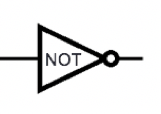
\includegraphics[height=0.5in]{../../resources/images/NOTx.png} \end{center}
%     \end{tabular}
%     \end{center}\end{document}